\chapter{Installation Mode} \label{Install_chapter}



\section{Installing for the First Time}
This toolbox are installed like any other Octave toolboxes. Consequently, the installation procedure is as detailed below.

\begin{enumerate}
	\item[\textbf{Step 1.}] Download the file \texttt{ltitool.tar.gz} To download the file for the first time you must go the website  \url{http://www.fiq.unl.edu.ar/control/index.php?page=software}.
	\item[\textbf{Step 2.}] Run the following command in the directory where the file was downloaded.
	\begin{verbatim}
		>>> pkg install ltitool.tar.gz
	\end{verbatim}
\end{enumerate}

In this way, the toolbox is already installed and ready to use. Then, write the following commands to execute the toolbox mentioned before:
	\begin{verbatim}
		>>> pkg load ltitool
		>>> ltitool
	\end{verbatim}

\section{Updating the Version}

If you already have LTITOOOL installed, then when a new version is available, a window like the one is shown in Fig. \ref{chp_install_fig01}.

\begin{figure}[H]
	\centering
	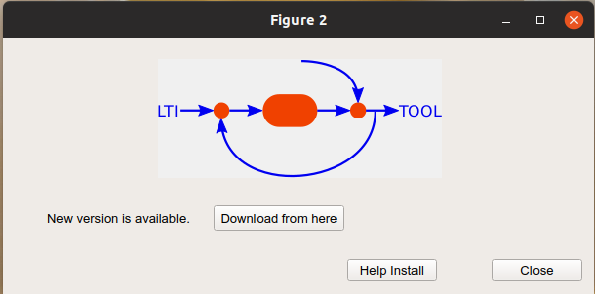
\includegraphics[scale=0.58]{./figuras/chapter_install/ltitoolNewVersionWnd.png}
	\caption{Updating to a new version.}
	\label{chp_install_fig01}
\end{figure}



Simply, you have to press the download button and then you have to follow the procedure indicated  below.
\begin{enumerate}
	\item[\textbf{Step 1.}] Uninstall the version you currently have installed. To do this, execute the command
	\begin{verbatim}
		>>> pkg uninstall ltitool.tar.gz
	\end{verbatim}
	Alternatively, it might be convenient to close and reopen Octave, but this should not be necessary.

	\item[\textbf{Step 2.}] Run the following command in the directory where the file was downloaded.
	\begin{verbatim}
		>>> pkg install ltitool.tar.gz
	\end{verbatim}
	
	Finally, you have the new version installed and to execute it you must follow the steps indicated in the previous section.
\end{enumerate}


 